\begin{tikzpicture}[x=.945cm,y=.95cm,font=\sitneoznake,>=Latex]
\node[anchor=west]at(4.7,2.65){N014};
\draw(.75,.95)--(.9,1.25)--(1.8,1.25)--(1.95,.95)--(1.8,.65)--(.9,.65)--cycle;
\draw(.75,.95)--(.6,.85)--(.45,.15)--(.55,.15)--(.7,.85)--(.8,.85);\draw(1.95,.95)--(2.1,.85)--(2.25,.15)--(2.15,.15)--(2,.85)--(1.9,.85);
\draw(1.15,1.25)--(1.2,1.17)--(1.5,1.17)--(1.55,1.25);
\draw[dashed](.4,.65)--(2.35,.65);\draw[->](2.4,.5)--(1.35,.65);\node[right]at(2.4,.5){SEATING PLANE};
\draw[<->](.6,2.2)--(2.1,2.2);\draw(.6,.85)--(.6,2.45);\draw(2.1,.85)--(2.1,2.45);\node[above]at(.6,2.45){$\mathrm{C\!L}$};\node[above]at(2.1,2.45){$\mathrm{C\!L}$};\node[right,align=left]at(2.3,2.2){7,62 $\pm$ 0,25\\(0.300 $\pm$ 0.010)};
\draw[<->](.75,1.8)--(1.95,1.8);\draw(.75,.95)--(.75,1.9);\draw(1.95,.95)--(1.95,1.9);\node[right,align=left]at(2.3,1.6){6,35 $\pm$ 0,25\\(0.250 $\pm$ 0.010)};
\draw[<->](1.15,1.48)--(1.55,1.48);\node[right]at(2.3,1.05){2,0 (0.080) NOM};\draw[->](2.3,1.05)--(1.35,1.48);
\draw[<->](1.7,1.25)--(1.7,1.17);\node[right]at(2.3,.78){0,25 (0.010) NOM};\draw[->](2.3,.78)--(1.7,1.2);
\node[below,align=left]at(1.2,-.05){\begin{tabular}{@{}l@{\quad}l@{}}105$^\circ$&\multirow{2}{*}{14 PLACES}\\90$^\circ$&\end{tabular}};\draw[->](.5,-.05)--(.5,.25);
\node[below]at(2.25,-.8){\begin{tabular}{@{}l@{\quad}l@{}}0,36 (0.014)&14 PLACES\\0,25 (0.010)&(See Notes B and C)\end{tabular}};\draw[<->](2.15,.05)--(2.25,.05);\draw(2.15,.15)--(2.15,-.02);\draw(2.25,.15)--(2.25,-.02);\draw[->](2.8,-.7)--(2.2,.05);
% Plan view, pin numbers and notch measurements.
\begin{scope}[shift={(4.7,0)}]
\draw(.25,.8)rectangle(3.45,1.5);\draw(.25,1.02)..controls(.7,1.02)and(.7,1.28)..(.25,1.28);
\foreach\i in{0,...,6}{\pgfmathtruncatemacro{\a}{14-\i}\pgfmathtruncatemacro{\b}{1+\i}\draw(.45+\i*.46,1.5)--++(0,.15);\draw(.45+\i*.46,.8)--++(0,-.15);\node[draw,circle,inner sep=.3pt]at(.45+\i*.46,1.86){\a};\node[draw,circle,inner sep=.3pt]at(.45+\i*.46,.45){\b};}
\draw[<->](.25,2.3)--(3.45,2.3);\draw(.25,1.5)--(.25,2.45);\draw(3.45,1.5)--(3.45,2.45);\node[above,align=center]at(1.85,2.3){19,8 (0.780)\\18,0 (0.710)};
\node[below,align=left]at(1.1,-.15){2,4 (0.093) R NOM\\2,8 (0.110) NOM};\draw[->](.6,-.1)--(.4,1.08);\draw[->](1.4,-.1)--(.4,1.23);
\node[anchor=north west]at(2.5,-.45){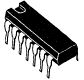
\includegraphics[height=1cm]{slike/izvorne/s075_fotografija_dip14.png}};
\end{scope}
% Front view and pin geometry; leaders preserve association of each dimension.
\begin{scope}[shift={(9.5,0)}]
\draw(.25,1.3)rectangle(3.55,1.8);\draw(.25,1.48)--(3.55,1.48);
\foreach\i in{0,...,6}{\draw(.4+\i*.47,1.3)--(.4+\i*.47,1.07)--(.46+\i*.47,.93)--(.46+\i*.47,.5)--(.56+\i*.47,.5)--(.56+\i*.47,.93)--(.62+\i*.47,1.07)--(.62+\i*.47,1.3);}
\draw[dashed](0,.98)--(3.8,.98);
\draw[<->](.1,1.8)--(.1,.98);\node[above,align=center]at(.8,2){5,08 (0.200) MAX};\draw[->](.8,2)--(.1,1.5);
\node[above,align=center]at(2.8,2.45){1,78 (0.070) MAX 14 PLACES};\draw[<->](.4,1.93)--(.62,1.93);\draw[->](2.5,2.4)--(.55,1.94);
\draw[<->](3.75,1.3)--(3.75,.98);\node[right,align=left]at(3.8,1.4){0,51\\(0.020)\\MIN};
\draw[<->](.1,.98)--(.1,.5);\node[left,align=right]at(.05,.5){3,17\\(0.125)\\MIN};
\node[below,align=left]at(1.6,.1){2,03 $\pm$ 0,51 (0.080 $\pm$ 0.020)\\4 PLACES};\draw[<->](.25,.25)--(.51,.25);\draw(.25,1.3)--(.25,.15);\draw(.51,.5)--(.51,.15);\draw[->](.85,.1)--(.38,.25);
\node[right,align=left]at(3.8,.2){0,84\\(0.033) MIN\\14 PLACES};\draw[<->](3.255,.98)--(3.405,.98);\draw[->](3.8,.2)--(3.33,.98);
\node[below]at(2.2,-.9){\begin{tabular}{@{}l@{\quad}l@{}}0,533 (0.021)&14 PLACES\\0,381 (0.015)&(See Notes B and C)\end{tabular}};\draw[<->](3.28,.35)--(3.38,.35);\draw[->](3.3,-.8)--(3.33,.35);
\draw[<->](.98,.32)--(1.45,.32);\draw[->](1.2,-1.15)--(1.24,.32);
\end{scope}\end{tikzpicture}
